\documentclass[twocolumn]{article}
\usepackage{graphicx}
\usepackage{fullpage}
\usepackage{amsmath}
\title{An approximation to the exponential function}
\author{J.T.~Madsen}
\date{}
\begin{document}
\maketitle

\begin{abstract}
An implementation of the exponential function is introduced
and compared to the standard exponential function from the math library.
\end{abstract}

\section{Introduction}
An exponential function is a type of function that is most often seen on the form,
	\begin{equation}\label{eq:exp}
f(x)=e^x \;.
	\end{equation}
This form is often seen since the derivative of $f(x)=f'(x)$ and this is a differential equation
often needed to be solved in e.g. physics. One of its characteristics is that it has a
well-defined half-life which can be used to describe e.g. radioactive decay.
One of many simple approximation to the function~(\ref{eq:exp}) is
a power series which is accurate for an infinite number of terms~\cite{rudin-walter},
	\begin{equation}\label{eq:walter}
\exp x := \sum_{k = 0}^{\infty} \frac{x^k}{k!}
 = 1 + x + \frac{x^2}{2} + \frac{x^3}{6} + \frac{x^4}{24} + \cdots
	\end{equation}
This can easily be seen as true by applying the power rule of differentiation.

\section{The implementation}
Our implementation reacts differently for x in different intervals. For negative x 
the reciprocal function is used which in general is possible for exponential functions since 
$a^{-b}=1/a^b$. 
Furthermore, the implementation evaluates values for x in the interval $[0,1/8]$
via the Tayler expansion to the 10th term.
The trick in this implementation is that for larger values of x 
it is used that $e^x=(e^{x/2})^2$. This is used recursively to propagate the error 
of the Taylor function. Let us say we wish to evaluate $e^{1/2}$. This would be 
reinterpreted as $(e^{1/8})^4$ and from here evaluated via the Taylor expansion.
This is a very clever way of propagating the error.


\section{The convoluted Taylor series}
For small values of x, the exponential function
is computed via the following implementatin:
	\begin{equation}\label{eq:Taylor}
	\begin{aligned}
\exp x \approx 1+x(1+x/2(1+x/3(1+x/4(1+x/5(1 \\
+x/6(1+x/7(1+x/8(1+x/9(1+x/10))))))))).
	\end{aligned}
	\end{equation}
This would work because every term in the series~(\ref{eq:Taylor})
can be made up of a product of the terms previous to it-only dividing by an integer
equal to 1 added to the number of terms previous to the term.
This is exactly why it is useful: it reuses the multiplication of the previous term
instead of doing the factorial from the ground up for every new term.

\section{Comparison}
Here is an illustration of the implementation, compared with the built-in
exponential function from the standard C-library.
It is seen that the overlap of the graphs are so large that only one of them is in fact seen.
This suggets a very large corelation between the two i.e. the approximation is good.


	\begin{figure}[h]
\centering
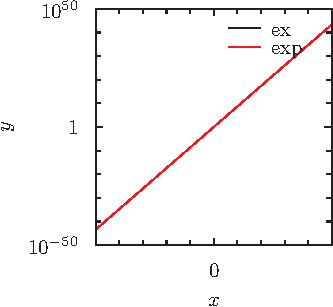
\includegraphics{fig-pyxplot.pdf}
\caption{Our implementation vs. C's implementation of the exponential function}
\label{fig:pyxplot}
	\end{figure}

\clearpage
\begin{thebibliography}{9}
\bibitem{rudin-walter} Rudin, Walter (1987). Real and complex analysis (3rd ed.).
New York: McGraw-Hill. p. 1. ISBN 978-0-07-054234-1,
\end{thebibliography}

\end{document}
